% IEEE ESL letter draft (4 pages). Compile on Overleaf with IEEEtran.
% Numbers marked <...> are filled from device measurements (2026-11-05/06).
\documentclass[journal,letterpaper]{IEEEtran}

\usepackage{cite}
\usepackage{amsmath,amssymb}
\usepackage{graphicx}
\usepackage{booktabs}
\usepackage{array}
\usepackage{url}

\begin{document}

\title{Fully-Resident Weight Storage for Mixed-Precision\\ SLM Inference on a 32-MB PSRAM MCU}

\author{Shizhou Xu%%
\thanks{Guangxi Medical University, Nanning, China; e-mail: X16717701114@outlook.com.
Manuscript received November 6, 2026.}}

\markboth{IEEE Embedded Systems Letters}%
{S.~Xu: Fully-Resident Weight Storage for Mixed-Precision SLM Inference}

\maketitle

\begin{abstract}
We show that mixed-precision quantization enables fully-resident weight storage of a dense
small language model (SLM) on a 32-MB PSRAM microcontroller. A 63.91M-parameter model
quantized to q3e4 (embedding/output q4, attention and FFN q3) occupies \textbf{27.3 MiB}
and runs entirely in on-board PSRAM with a \textbf{192-token} context window (FP16 K/V cache)
and no PC host at inference time. Measured decode throughput is \textbf{0.620 tok/s}
(1.61 s/token) after int16-activation, zero-copy packed GEMV, activation-quantization hoisting,
and a 32-bit batch-unpack / four-way-unrolled / \texttt{-O3} pass, a \textbf{3.62$\times$}
cumulative speedup over a row-expanded fp32 baseline re-measured on the same board
(2.21$\times$ format/activation change, 1.23$\times$ hoisting, 1.33$\times$ unpack); the GEMV
kernel dominates decode time, so kernel-level gains pass through almost unchanged to decode
latency. A pre-registered screening bound (fixed-text cross-entropy within 1.15$\times$ of q4,
plus a deterministic 30-prompt well-formedness score $\geq 80\%$) is met by q3e4 on the host
recipe (24/30; device 22/30) while mixed and the smaller variants fail the rule criterion; q3e4
keeps about 40$\times$ more PSRAM headroom at runtime and is selected for deployment. All
arithmetic is documented and reproducible from the open artifact.
\end{abstract}

\begin{IEEEkeywords}
Edge AI, on-device inference, large language models, mixed-precision quantization, PSRAM.
\end{IEEEkeywords}

\section{Introduction}
\IEEEPARstart{P}{utting} an entire dense language model on a microcontroller is a capacity
problem before it is a compute problem. On a fixed 32-MB PSRAM budget, a 63.91M-parameter
SLM needs about 122~MiB in FP16 and 61~MiB in INT8 (244~MiB in FP32), all far beyond on-board memory;
weights must therefore be compressed until they fit, and any configuration that does not fit
is simply not a candidate, regardless of its arithmetic quality.

Prior work avoids this wall~\cite{memorywall} in two ways. A 180.9M-parameter MoE design (p-for-llm)~\cite{pforllm} trades
dense residency for sparsity: only the routed experts are active, its $\sim$44~MiB of state
is split between flash XIP and PSRAM, and part of the PSRAM weights are transferred from a
host over USB at boot, so the host is absent during inference yet still required at startup;
its $\sim$9~tok/s reflects top-1 routing over 29 experts per layer. The PIE series~\cite{pie} instead
accelerates kernels on models far below the capacity boundary (0.61$\rightarrow$4.31~tok/s)
and does not address how much dense model can reside. A recent survey of MCU LLM systems~\cite{survey}
finds fully-on-chip evidence only at the 256--412~KB scale and one 5.81~MB ternary ViT~\cite{ternaryvit} with
external PSRAM; a fully-resident \emph{dense} 27.3~MiB model on an ESP32-class device falls
in a region that is not covered. For scale, an ESP32-S3 board has been reported at 22.6~tok/s on a TinyStories-scale model~\cite{edgebench}.

This letter answers two questions within one concrete design point: how far a dense SLM can be
compressed and still reside fully in 32~MB of PSRAM, and what latency that residency costs once
the storage problem is solved. We quantify the deployment frontier with a pre-registered
accuracy bound, measure the decode-time split between GEMV and the rest of the forward pass,
and show that the GEMV kernel---not PSRAM bandwidth---dominates latency, which is why
kernel-level gains from 2.21$\times$ to 3.62$\times$ appear almost one-to-one at the system level. We do not claim a new
quantization method or a new system architecture: the contribution is an auditable capacity point,
a measured latency-cost attribution, and a reproducible artifact.

\section{Method}
\textbf{Quantization scheme.} Following the group-wise post-training quantization line~\cite{gptq,awq,llmint8}, q3e4 stores the token embedding and the tied output layer at
q4\_0 (18 bytes per 32 weights: one fp16 block scale plus 16 packed nibbles) and all attention
and FFN linear projections at q3\_0 (14 bytes per 32 weights: fp16 scale plus 12 packed
3-bit values). Activations are quantized to int16 per GEMV call~\cite{int16}; RMSNorm weights and biases remain FP32; the deployed K/V cache is FP16 at 192 tokens (Sec.~III). A KMCU image is a single flat file with a 4,480-byte header followed
by per-tensor packed blocks; the q3e4 image is 28,632,448 bytes (27.3~MiB).

\textbf{Accuracy bound (pre-registered).} A configuration is deployable only if it
simultaneously satisfies (i) per-token cross-entropy on a fixed text within 1.15$\times$ of the
q4 reference, and (ii) a deterministic well-formedness score of at least 80\% on 30 fixed
prompts (length, repetition, ending, echo and control-character rules). The thresholds, prompt
set and rule checker were fixed before any q3e4 measurement and are archived in the artifact at
commit \texttt{be624d7} (2026-11-05, 3.6~h before the first q3e4 device log); they are not
adjusted afterwards. Because the frontier is host-simulated, the score is evaluated with the
host recipe, and the device score of the deployed image is reported as a cross-check. The q4
reference cannot run on the device (36.0~MB exceeds the budget), so it is simulated on a host
with the identical block-32 recipe.

\textbf{Bit allocation rationale.} The embedding and output matrix (6400$\times$768) is kept at
q4 because it carries lexical identity and is reused by the tied head; attention and FFN are both
q3 in q3e4 (the mixed variant promotes attention to q4). The all-q3 variant is 0.61~MB smaller
with nearly identical CE, but it scores 21/30 = 70\% on the rule set, below the 80\% gate, so
keeping the embedding/output at q4 is justified by the rule criterion rather than by CE alone.

\textbf{Zero-copy packed GEMV.} Dequantizing to an expanded copy would multiply the resident
footprint (8.5$\times$ for FP32, 2.1$\times$ for INT8) and add per-element traffic. Instead, the
packed image is used in place: each 32-weight block is read from PSRAM, unpacked on the fly into
signed integers, and dotted with the int16 activation vector; the fp16 block scale is applied to
the integer partial sum. The inner loops unpack eight 3-bit fields from three bytes with constant
shifts, keep four independent integer accumulators, and process two output rows per pass; the
final build adds \texttt{-O3}. Our implementation builds on the Kestrel-MCU engine~\cite{kestrel}:
the q4\_0/q3\_0 formats and packed GEMV are reused, while the int16 integer path, 3-bit unpack,
quantization hoisting, block-sum correction, two-row unrolling and FP16 K/V cache are new.
Kestrel's optional PIE w8a16 path expands weights to int8 (61~MB here), which cannot fit the
32-MB budget; packed 3-bit storage is the binding constraint.

\textbf{Context and KV budget.} The deployed context is 192 tokens with FP16 K/V caches:
$2 \times 8 \times 192 \times 4 \times 96 \times 2$~B $=$ 2,359,296~B, i.e. the same PSRAM as a
96-token FP32 cache (for reference, 96 tokens with FP32 K/V was the earlier configuration;
Sec.~III reports the measured effect of the FP16 cache).

\textbf{Model and board.} The 63.91M model (8 layers, hidden 768, 8 query / 4 KV heads of 96,
FFN 2432, vocab 6400 tied) is trained from scratch on a local 12-GB GPU on the public MiniMind
dataset (ModelScope \texttt{gongjy/minimind\_dataset}): pre-training (39,695 steps, final loss
2.01) and supervised fine-tuning (56,608 steps, final loss 1.71), then quantized to q3e4. The
architecture follows Qwen3-style QK-norm~\cite{qwen3} and the MiniMind recipe~\cite{minimind};
a QK-norm correction in the deployed kernel is an enabling fix, not a contribution. The target
board is an ALINTEK ESP32-P4 (360~MHz, 16~MB flash, on-board 32~MB PSRAM)~\cite{psram}; the
image and tokenizer are loaded once from a microSD card, and the board serves as a local AI endpoint for a HachimoDock desktop pet~\cite{hachimodock}.


\section{Results}
\textbf{Memory budget (Table~\ref{tab:budget}).} All weights and caches are allocated once at
boot and their sizes are auditable: the q3e4 image (28,632,448~B), the FP16 K/V cache
(2,359,296~B), 209,860~B of runtime PSRAM used by the SD/VFS layer and heap, and 538,656~B of
tokenizer tables leave \textbf{1,814,172~B free at ready}, measured at runtime (the free space
after K/V initialization alone is 2,352,828~B). A mixed image (30,401,920~B) leaves only 44,700~B
at ready.

\begin{table}[t]
\centering
\caption{Deployed PSRAM budget on a 32-MB PSRAM ESP32-P4 (measured). The small norm arena and scratch buffers live in internal RAM and are outside this table; rows sum to 33,554,432~B.}
\label{tab:budget}
\footnotesize
\setlength{\tabcolsep}{2.5pt}
\begin{tabular}{@{}lr@{}}
\toprule
Item & Bytes \\
\midrule
q3e4 weights & 28,632,448 (27.3 MiB) \\
KV (192 tok, FP16) & 2,359,296 \\
Runtime PSRAM (SD/VFS, heap) & 209,860 \\
Tokenizer tables & 538,656 \\
\midrule
Free at ready & 1,814,172 \\
\midrule
PSRAM total & $\leq$ 33,554,432 \\
\bottomrule
\end{tabular}
\end{table}

\begin{figure*}[t]
\centering
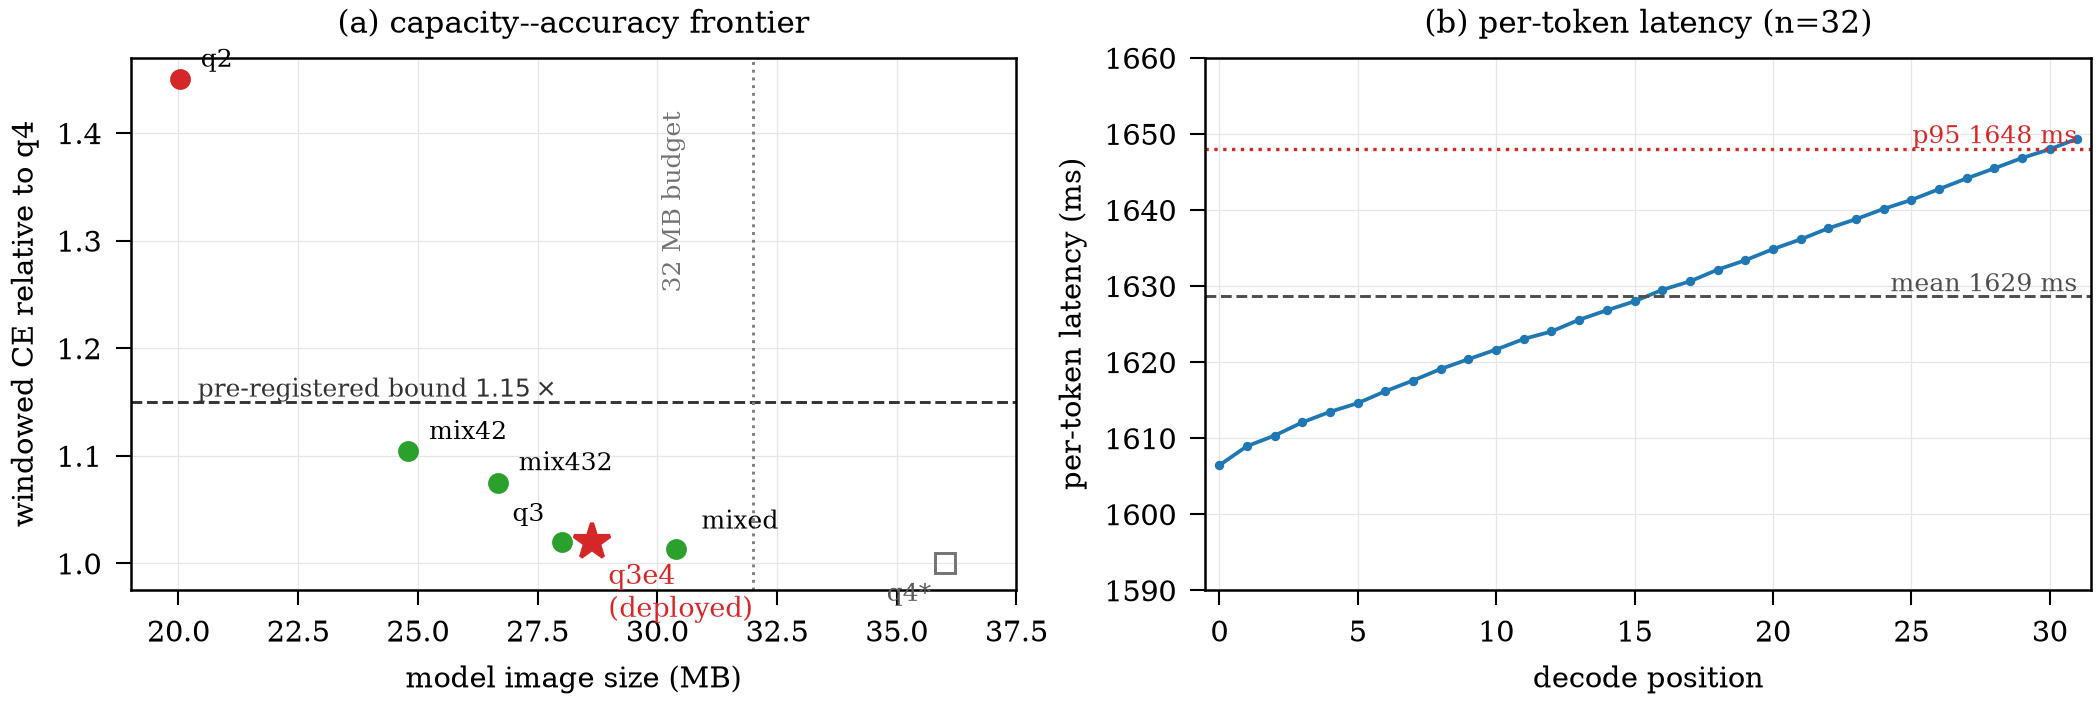
\includegraphics[width=\textwidth]{figures/fig_frontier_latency.png}
\caption{(a) Capacity--accuracy frontier: windowed CE relative to q4 versus model image size.
The $1.15\times$ line is the CE criterion; the dotted line is the image budget left after the
192-token KV cache, runtime allocations and tokenizer tables (30.45~MB). q3e4 is the only configuration that also
passes the rule criterion on the host recipe. q4$^*$ is the CE reference (36.0~MB, does not
fit). (b) Distribution of per-token decode latency over 64 measured steps (mean 1,620.5~ms,
p95 1,645.5~ms).}
\label{fig:frontier}
\end{figure*}

\textbf{Decode latency and GEMV share (Table~\ref{tab:gemv}, Fig.~\ref{fig:frontier}b).}
The baseline is the earlier row-expanded fp32 path: each weight row is expanded into a
4,096-float buffer before the dot product, so only one row is ever resident and the full model is
never expanded. Replacing it with int16 activations and integer packed weights reduces decode
from 5,833 to 2,639~ms/token (0.379~tok/s, 2.21$\times$). Hoisting the per-token activation
quantization out of the 6,400-row output-head loop and replacing per-weight offsets by block-sum
corrections reaches 2,152~ms/token (0.465~tok/s), and the 32-bit batch-unpack / four-way /
\texttt{-O3} pass reaches \textbf{1,612~ms/token (0.620~tok/s)}, i.e. 3.62$\times$ cumulative.
Cycle counters give GEMV shares $r=0.988$, 0.985 and 0.977 on the three packed builds; Amdahl's
law with these shares and the measured cleanup-stage gains (1.23$\times$, 1.33$\times$) predicts
1.22$\times$ and 1.32$\times$ versus 1.23$\times$ and 1.33$\times$ observed. Counting one full
read of packed weights (28.63~MB) plus one complete KV pass (2.36~MB) gives 30.99~MB/token, i.e.
11.7, 14.4 and 19.2~MB/s for the three packed builds (weight-only 10.98, 13.5 and 18.2~MB/s),
far below the 95.9~MB/s sequential-read microbenchmark (1~MB buffer, four accumulators). To
separate memory traffic from instruction cost, a read-only variant that streams the same packed
bytes without unpacking or dot products runs at \textbf{600~ms/token} (GEMV 519~ms, 55~MB/s),
while the real GEMV costs 1,575~ms: about two thirds of decode time is the unpack/integer-dot
instruction stream rather than PSRAM traffic.

\begin{table}[t]
\centering
\caption{Decode-time ablation (device; first row re-measured on the same board and model).}
\label{tab:gemv}
\footnotesize
\setlength{\tabcolsep}{2.5pt}
\begin{tabular}{@{}lrrrr@{}}
\toprule
Config & ms/tok & Speedup & $r$ & MB/s \\
\midrule
Row-expanded fp32 & 5,833 & 1$\times$ & -- & -- \\
int16 + packed & 2,639 & 2.21$\times$ & 0.988 & 10.98 \\
+ hoisted quant. & 2,152 & 2.71$\times$ & 0.985 & 13.5 \\
+ batch unroll, \texttt{-O3} & \textbf{1,612} & \textbf{3.62$\times$} & 0.977 & 18.2 \\
\bottomrule
\end{tabular}
\end{table}

\textbf{FP16 K/V cache.} Storing the K/V cache in FP16 doubles the context from 96 to 192
tokens at the same 2,359,296~B. On the same prefix, window-0 CE changes from 6.662094 to
6.660668 ($\Delta=0.0014$, 0.02\%) and decode time stays within run-to-run variation (measured
on the pre-optimization kernel), so the larger context is adopted at no measurable accuracy
cost. The context change itself has a large modeling effect: one 192-token window scores CE
5.970 versus 7.014 for resetting every 96 tokens (PPL 392 vs.\ 1,112), i.e. about a 15\%
reduction in CE.

\textbf{Accuracy frontier (Table~\ref{tab:frontier}, Fig.~\ref{fig:frontier}a).} Host
simulation with the identical 96-token windowed recipe places q4 at CE $=6.949$ (PPL 1,042) and
q3e4 at 7.087 (1.020$\times$, PPL 1,197); q2 reaches 10.074 (1.450$\times$, PPL 23,710). On
the English corpus (Apache-2.0 text, 288 tokens) the ordering is unchanged: q3e4 5.676
(1.048$\times$) versus q2 9.905 (1.829$\times$). With 192-token windows the ratios are
q3e4/q4 $=1.021$, mixed $=1.008$, q3 $=1.024$ and q2 $=1.611$, so the ranking is insensitive to
the evaluation window. The 30-prompt well-formedness score is 24/30 (80\%) for q3e4 on the host
recipe, 22/30 (73.3\%) on the device run, 21/30 for q3, 22/30 for mixed and q4, and 0/30 for q2;
an extended 100-prompt set gives 63\% for q3e4 (95\% CI 53--72) versus 66\% for fp32, 68\% for
mixed and 0\% for q2, while a coarse task check on that set's math/code/translation subsets
yields only 1/10, 5/10 and 1/10 correct for every non-degenerate configuration. The
pre-registered 80\% gate is therefore a screening criterion on the fixed 30-prompt set, not a
general accuracy estimate. On the same held-out corpora the public MiniMind-3 checkpoint scores
CE 7.41 (Chinese) and 6.28 (English) versus 6.97 and 5.40 for our model. Only q3e4 passes the
screening gate on the host recipe: mixed meets the CE criterion (7.037, 1.013$\times$) but fails
the rule gate (22/30) and leaves only 44,700~B at ready, whereas q3e4 leaves 1,814,172~B (about
40$\times$ more); mix42 and mix432 meet CE but fail the rule gate (18/30 and 20/30).

\begin{table}[t]
\centering
\caption{Capacity--accuracy frontier (32-MB PSRAM). Sizes, CE and rule scores are host-simulated with the identical windowed recipe; the last column is device decode time on the final build.}
\label{tab:frontier}
\footnotesize
\setlength{\tabcolsep}{2.5pt}
\begin{tabular}{@{}lrrrrr@{}}
\toprule
Config & Size (B) & CE & CE/q4 & Rule & ms \\
\midrule
q2 & 20,030,848 & 10.074 & 1.450 & 0\% & 1,352 \\
q3 & 28,018,048 & 7.090 & 1.020 & 70\% & -- \\
\textbf{q3e4} & \textbf{28,632,448} & \textbf{7.087} & \textbf{1.020} & \textbf{80\%} & \textbf{1,612} \\
mixed & 30,401,920 & 7.037 & 1.013 & 73.3\% & 2,017 \\
q4 & 36,005,248 & 6.949 & 1.000 & 73.3\% & n/a \\
fp32 & -- & 6.973 & 1.003 & 80\% & n/a \\
\bottomrule
\end{tabular}
\end{table}



\textbf{Positioning (Table~\ref{tab:compare}).} The closest points are a sparsity-assisted MoE
with partial residency and a boot-time host transfer, and vector-kernel acceleration on models
well below the capacity boundary. We do not compare throughput directly: the table positions
constraint differences, and the reported throughputs are cited as reported by their authors.

\begin{table}[t]
\centering
\caption{Constraint comparison. Prior-work throughputs are as reported by their authors; this work is measured on the final build.}
\label{tab:compare}
\footnotesize
\setlength{\tabcolsep}{2.5pt}
\begin{tabular}{@{}lrrr@{}}
\toprule
Work & Model & Residency / boot & tok/s \\
\midrule
p-for-llm & 180.9M MoE & partial; USB boot & $\sim$9 \\
PIE & -- & kernel accel.; no capacity & 0.61--4.31 \\
\textbf{This work} & 63.91M dense & \textbf{full 27.3 MiB; no PC host} & \textbf{0.620} \\
\bottomrule
\end{tabular}
\end{table}

\textbf{Decode and startup.} Weight loading from a TF card takes about 20.6~s, dominated by the
card read (the packed image needs no post-load unpacking). A 32-token run gives mean 1,629~ms and
p95 1,648~ms, and a 64-step measurement gives mean 1,620.5~ms, median 1,616.0~ms, p95
1,645.5~ms (std.\ 12.4~ms), i.e. a narrow distribution without long tails; latency rises by about
2.7\% from position 0 to 31 as attention reads a longer K/V cache. Prompt prefill is processed
token-by-token (no batched prefill), so a short query plus a 32-token reply takes on the order of
one to two minutes. The mixed configuration (30.40~MB) also boots and generates in the full
standalone firmware, confirming that it is deployable; the other frontier variants were evaluated
on the host only.

\section{Discussion and Limitations}
The measured split changes the design story: the deployment is GEMV-bound ($r=0.977$ in the
final build), and the unpack/dot instruction stream is the throughput limiter, not the PSRAM
bandwidth. The practical consequence is that kernel work survives at the system level
(3.62$\times$ cumulative); the final build costs about 9.1 cycles per weight
(360~MHz $\times$ 1.612~s / 63.9M) versus 32.9 cycles for the row-expanded baseline, and the
read-only control above shows that the same bytes can be streamed in 600~ms/token---so the
remaining cost is the unpack/integer-dot instruction stream. Wider unpacking has already been
applied, so further gains would require a different core/ISA or custom instructions rather than
fewer bytes read. The 192-token context is obtained at no extra memory by storing the K/V cache in FP16
(2.25~MiB for 192 tokens); measured windowed CE changes by 0.0014 and decode time stays within run-to-run variation on
the pre-optimization kernel, so the FP16 cache is adopted for deployment while FP32 K/V at 96
tokens remains a conservative fallback. The absolute format-validity rate (~65\% on the
100-prompt set) and the absence of a standard benchmark remain the main limitations of the
evaluation. The model itself is deliberately small and trained on a single local GPU; its absolute
quality is not the claim---accuracy measurements only delimit the feasible set. We report no
energy-per-token figure (no power meter was available) and no standard benchmark score; a fixed
held-out text and a deterministic rule set keep the comparison auditable but bound external
validity. The usage model is single-turn: prompt prefill is token-by-token and replies are
short, so the reported throughput is not a conversational latency. The artifact,
training logs, evaluation scripts and the self-trained q3e4 image are public for reproduction.

\textbf{Reproducibility and artifact.} The public repository
\url{https://github.com/KAYOYAK/hachimodock-minimind-esp32p4} (release v0.2.1) contains the
self-trained q3e4 image (SHA-256
\texttt{feb574f966980a71c53c6b1f56daf054f}\allowbreak\texttt{267ed425b72ee5ce93f6002ccf87f0}), the firmware
sources, the 30- and 100-prompt sets with the rule checker, the windowed-CE and checkpoint
scripts, and all six alternative images. Every number in Tables~I--III and the this-work row of
Table~IV can be regenerated from these files; the host simulation uses the identical block-32
recipe, and the host/device agreement above bounds its error for the configurations that run on
both sides.

\section{Conclusion}
A 63.91M dense SLM can reside fully in 32~MB of PSRAM at 27.3~MiB with a 192-token context and
no PC host, and decode latency is dominated by the packed GEMV instruction stream rather than
memory bandwidth, so kernel-level work transfers almost directly to decode speed. The
0.620~tok/s figure is decode-only: boot takes about 20.6~s, prefill is token-by-token, and the
device is used for short single-turn queries. The capacity--accuracy frontier, with q2 beyond
the budget and q4 beyond the capacity, is measured under a pre-registered screening bound and is
reproducible from the public artifact.

\section*{Acknowledgment}
The author used the DeepSeek Harness AI coding agent (DeepSeek model) to assist with the
ESP32-P4 firmware implementation (model loading, packed-weight GEMV kernels, USB host protocol
bridge), quantization and measurement tooling (Sections II--III), experiment automation, and
manuscript editing. The AI system is not an author. The author independently verified all
generated code, measurements and text and takes full responsibility for the accuracy,
originality and integrity of this work. This work received no external funding, and the author
declares no conflict of interest.

\begin{thebibliography}{18}
\bibitem{pforllm} cyfrit, ``PFor: Offline 180.9M-parameter LLM and agent inference on ESP32-P4,'' GitHub repository, 2026. [Online]. Available: https://github.com/cyfrit/p-for-llm
\bibitem{pie} ``From 0.61 to 4.31 tok/s: A complete record of MCU-side LLM inference level-four optimization,'' EEWorld forum, Oct. 2026. [Online]. Available: \url{https://en.eeworld.com.cn/bbs/forum.php?mod=viewthread&tid=1369555}
\bibitem{kestrel} m13253246268-ship-it, ``Kestrel-MCU: an Apache-2.0 LLM inference engine for RISC-V MCUs,'' GitHub repository, 2026. [Online]. Available: https://github.com/m13253246268-ship-it/kestrel-llm-mcu
\bibitem{survey} M.~R.~Ramdhani, ``Language and transformer models with ESP32-class microcontrollers: A systematic review of hybrid deployment and on-device optimization,'' 2026. [Online]. Available: https://journals.unpad.ac.id/ijmt/article/view/72405
\bibitem{qwen3} Qwen Team, ``Qwen3 technical report,'' arXiv:2505.09388, 2025.
\bibitem{gptq} G.~Frantar, S.~Ashkboos, T.~Hoefler, and D.~Alistarh, ``GPTQ: Accurate post-training quantization for generative pre-trained transformers,'' in \emph{Proc. ICLR}, 2023.
\bibitem{awq} J.~Lin \emph{et al.}, ``AWQ: Activation-aware weight quantization for on-device LLM compression and acceleration,'' in \emph{Proc. MLSys}, 2024.
\bibitem{llmint8} T.~Dettmers, M.~Lewis, Y.~Belkada, and L.~Zettlemoyer, ``LLM.int8(): 8-bit matrix multiplication for transformers at scale,'' in \emph{Proc. NeurIPS}, 2022.
\bibitem{psram} Espressif Systems, ``ESP32-P4 technical reference manual,'' 2025.
\bibitem{minimind} Jingyaogong, ``MiniMind: train a small language model from scratch,'' GitHub repository, 2025. [Online]. Available: https://github.com/jingyaogong/minimind
\bibitem{memorywall} W.~Wulf and S.~McKee, ``Hitting the memory wall: Implications of the obvious,'' \emph{ACM SIGARCH Comput. Archit. News}, vol.~23, no.~1, pp.~20--24, 1995.
\bibitem{edgebench} ``LLM on a microcontroller: ESP32-S3 at 22.6 tok/s,'' technical report, 2026. [Online]. Available: https://insiderllm.com/pdfs/llm-on-microcontroller-esp32-s3.pdf
\bibitem{int16} B.~Jacob \emph{et al.}, ``Quantization and training of neural networks for efficient integer-arithmetic-only inference,'' in \emph{Proc. CVPR}, 2018.
\bibitem{ternaryvit} S.~Ma, H.~Wang, L.~Ma, L.~Wang, W.~Wang, S.~Huang, L.~Dong, R.~Wang, J.~Xue, and F.~Wei, ``The era of 1-bit LLMs: All large language models are in 1.58 bits,'' arXiv:2402.17764, 2024.
\bibitem{hachimodock} Y.~Wang \emph{et al.}, ``HachimoDock: An open-source desktop AI hardware,'' GitHub repository, 2026. [Online]. Available: https://github.com/YizhengWw/HachimoDock
\end{thebibliography}

\end{document}
